\newpage

\section{Le Théorème Central Limite (TCL)}

\subsection{Introduction : L'omniprésence de la loi normale}

Dans la section précédente, la Loi des Grands Nombres (LLN) nous a donné une garantie fondamentale : la moyenne d'échantillon $\bar{X}_n$ converge vers la vraie moyenne $\mu$ lorsque $n$ devient grand.
$$ \bar{X}_n \xrightarrow{p.s.} \mu $$
La LLN nous dit \textbf{où} la moyenne d'échantillon converge (vers la constante $\mu$), mais elle ne nous dit rien sur la \textit{forme} de la distribution de $\bar{X}_n$ autour de $\mu$ pour un $n$ grand, mais fini.

Le \textbf{Théorème Central Limite (TCL)} comble cette lacune. Il décrit la \textit{manière} dont $\bar{X}_n$ converge, en nous donnant la forme de sa distribution. C'est sans doute le théorème le plus important des statistiques.

\begin{intuitionbox}[L'Idée Fondamentale]
Intuitivement, ce résultat affirme qu'une \textbf{somme} d'un grand nombre de variables aléatoires indépendantes et identiquement distribuées (i.i.d.) tend, le plus souvent, à suivre une \textbf{loi normale} (aussi appelée loi de Laplace-Gauss ou "courbe en cloche").

Ce théorème et ses généralisations offrent une explication à l'omniprésence de la loi normale dans la nature. De nombreux phénomènes (la taille d'un individu, l'erreur de mesure d'un instrument, le bruit de fond d'un signal) sont le résultat de l'addition d'un très grand nombre de petites perturbations aléatoires. Le TCL nous dit que le résultat de cette somme sera, inévitablement, distribué selon une loi normale.
\end{intuitionbox}

\subsection{L'illustration : la somme des "Pile ou Face"}

Prenons l'exemple le plus simple pour illustrer ce phénomène : le jeu de "pile ou face".



\begin{examplebox}[Distribution de la Somme de $n$ Lancers]
Soit $X_i$ le résultat du $i$-ème lancer, avec $X_i = 1$ pour "Face" (probabilité 0,5) et $X_i = 0$ pour "Pile" (probabilité 0,5). La distribution d'origine (pour $n=1$) n'est pas du tout une courbe en cloche : c'est une distribution discrète avec deux bâtons de même hauteur.

Considérons la \textbf{somme} $S_n = X_1 + X_2 + \dots + X_n$, qui représente le nombre total de "Face" obtenus en $n$ lancers.

\begin{itemize}
    \item \textbf{Pour $n=1$ :} La distribution de $S_1$ est :
    \begin{itemize}
        \item Valeurs de la somme : \{0, 1\}
        \item Fréquences : \{0.5, 0.5\}
    \end{itemize}
    
    \item \textbf{Pour $n=2$ :} Les sommes possibles sont \{0, 1, 2\}. La distribution de $S_2$ est :
    \begin{itemize}
        \item Valeurs de la somme : \{0, 1, 2\}
        \item Fréquences : \{0.25, 0.5, 0.25\} (elle forme un triangle).
    \end{itemize}
    
    \item \textbf{Pour $n=3$ :} Les sommes possibles sont \{0, 1, 2, 3\}. La distribution de $S_3$ est :
    \begin{itemize}
        \item Valeurs de la somme : \{0, 1, 2, 3\}
        \item Fréquences : \{0.125, 0.375, 0.375, 0.125\}
    \end{itemize}
\end{itemize}

\begin{center}
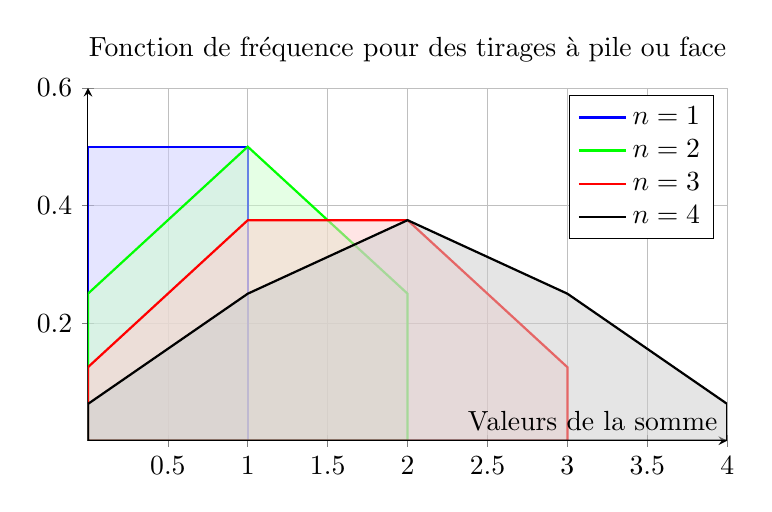
\begin{tikzpicture}
  \begin{axis}[
    width=0.8\textwidth,
    height=0.5\textwidth,
    xlabel={Valeurs de la somme},
    title={Fonction de fréquence pour des tirages à pile ou face},
    grid=both,
    grid style={line width=.1pt, draw=gray!30},
    major grid style={line width=.2pt,draw=gray!50},
    domain=0:4,
    samples=100,
    enlargelimits=false,
    axis lines=middle,
    xmin=0, xmax=4,
    ymin=0, ymax=0.6
  ]
  % n=1
  \addplot [thick, color=blue, fill=blue!20, fill opacity=0.5] coordinates {(0,0.5) (1,0.5)} \closedcycle;
  % n=2
  \addplot [thick, color=green, fill=green!20, fill opacity=0.5] coordinates {(0,0.25) (1,0.5) (2,0.25)} \closedcycle;
  % n=3
  \addplot [thick, color=red, fill=red!20, fill opacity=0.5] coordinates {(0,0.125) (1,0.375) (2,0.375) (3,0.125)} \closedcycle;
  % n=4 (suggéré)
  \addplot [thick, color=black, fill=black!20, fill opacity=0.5] coordinates {(0,0.0625) (1,0.25) (2,0.375) (3,0.25) (4,0.0625)} \closedcycle;
  
  \legend{$n=1$,$n=2$,$n=3$,$n=4$}
  \end{axis}
\end{tikzpicture}
\end{center}

Graphiquement, on constate que plus le nombre de tirages $n$ augmente (par exemple, jusqu'à $n=12$), plus la courbe de fréquence (qui reste discrète) se rapproche d'une courbe en cloche symétrique, caractéristique de la loi normale.
\end{examplebox}

\subsection{Distribution de la population vs. Distribution d'échantillonnage}

Le point le plus remarquable du TCL est qu'il fonctionne \textit{quelle que soit} la distribution de départ.

\begin{intuitionbox}[Population vs. Échantillonnage]
Imaginez deux univers de distributions :

\begin{itemize}
    \item \textbf{1. La Distribution de la Population ($X_i$) :} C'est la loi de nos variables $X_i$ individuelles. Elle peut avoir \textbf{n'importe quelle forme} (par exemple, une distribution bimodale, asymétrique, ou uniforme). Cette distribution a une "vraie" moyenne $\mu$ et un "vrai" écart-type $\sigma$.
    
    \item \textbf{2. La Distribution d'Échantillonnage ($\bar{X}_n$) :} C'est la distribution de la \textit{moyenne} $\bar{X}_n = (X_1 + \dots + X_n)/n$, calculée sur des échantillons de taille $n$. C'est la distribution de "toutes les moyennes d'échantillon possibles".
\end{itemize}

Le TCL énonce la relation magique entre les deux :

\textbf{Quelle que soit la forme de la distribution de la population, plus la taille de l'échantillon $n$ croît, plus la distribution d'échantillonnage de la moyenne $\bar{X}_n$ est proche d'une loi normale (gaussienne).}

De plus, les paramètres de cette loi normale sont :
\begin{itemize}
    \item \textbf{Moyenne :} La distribution de $\bar{X}_n$ est centrée sur la même moyenne $\mu$ que la population.
    \item \textbf{Écart-type :} La distribution de $\bar{X}_n$ est beaucoup plus resserrée. Son écart-type (appelé "erreur standard") est $\sigma_{\bar{X}} = \frac{\sigma}{\sqrt{n}}$.
\end{itemize}
Cette dispersion $\sigma/\sqrt{n}$ qui tend vers 0 est la manifestation de la Loi des Grands Nombres. Le TCL précise que la \textit{forme} de cette convergence est gaussienne.
\end{intuitionbox}

\subsection{Énoncé formel du Théorème Central Limite}

Pour énoncer le théorème formellement, nous devons d'abord définir les propriétés de la somme $S_n$ et de la moyenne $\bar{X}_n$.

Soit $X_1, \dots, X_n$ des variables aléatoires i.i.d. avec $E[X_i] = \mu$ et $\text{Var}(X_i) = \sigma^2$.

\begin{itemize}
    \item \textbf{La Somme $S_n = \sum X_i$} :
    \begin{itemize}
        \item Espérance : $E[S_n] = E[\sum X_i] = \sum E[X_i] = n\mu$
        \item Variance : $\text{Var}(S_n) = \text{Var}(\sum X_i) = \sum \text{Var}(X_i) = n\sigma^2$
        \item Écart-type : $\sigma_{S_n} = \sqrt{n\sigma^2} = \sigma\sqrt{n}$
    \end{itemize}
    
    \item \textbf{La Moyenne $\bar{X}_n = S_n / n$} :
    \begin{itemize}
        \item Espérance : $E[\bar{X}_n] = E[S_n / n] = \frac{1}{n} E[S_n] = \frac{1}{n} (n\mu) = \mu$
        \item Variance : $\text{Var}(\bar{X}_n) = \text{Var}(S_n / n) = \frac{1}{n^2} \text{Var}(S_n) = \frac{1}{n^2} (n\sigma^2) = \frac{\sigma^2}{n}$
        \item Écart-type : $\sigma_{\bar{X}_n} = \sqrt{\sigma^2 / n} = \frac{\sigma}{\sqrt{n}}$
    \end{itemize}
\end{itemize}

Nous voyons que la distribution de $S_n$ s'étale (variance $\to \infty$) tandis que celle de $\bar{X}_n$ se contracte (variance $\to 0$). Pour étudier la \textit{forme} de la convergence, nous créons une variable "stable" en la centrant (soustrayant la moyenne) et en la réduisant (divisant par l'écart-type). C'est la variable $Z_n$.

\begin{theorembox}[Théorème Central Limite (Lindeberg-Lévy)]
Soit $X_1, X_2, \dots, X_n$ une suite de variables aléatoires \textbf{i.i.d.} (indépendantes et identiquement distribuées) suivant la même loi $D$.
Supposons que l'\textbf{espérance $\mu$} et l'\textbf{écart-type $\sigma$} de cette loi $D$ existent, sont finis, et $\sigma \neq 0$.

Considérons la variable aléatoire standardisée $Z_n$ :
$$ Z_n = \frac{S_n - E[S_n]}{\sigma_{S_n}} = \frac{S_n - n\mu}{\sigma\sqrt{n}} $$
Cette variable est équivalente à la moyenne standardisée :
$$ Z_n = \frac{\bar{X}_n - E[\bar{X}_n]}{\sigma_{\bar{X}_n}} = \frac{\bar{X}_n - \mu}{\sigma / \sqrt{n}} $$
(Pour tout $n$, $Z_n$ est une variable centrée-réduite : $E[Z_n] = 0$ et $\text{Var}(Z_n) = 1$).

Alors, la suite de variables aléatoires $Z_1, Z_2, \dots, Z_n, \dots$ \textbf{converge en loi} vers une variable aléatoire $Z$ qui suit la \textbf{loi normale centrée réduite $N(0, 1)$}, lorsque $n$ tend vers l'infini.

Cela signifie que si $\Phi$ est la fonction de répartition de la loi $N(0, 1)$, alors pour tout réel $z$ :
$$ \lim_{n \to \infty} P(Z_n \le z) = \lim_{n \to \infty} P\left( \frac{\bar{X}_n - \mu}{\sigma/\sqrt{n}} \le z \right) = \Phi(z) $$
\end{theorembox}

\subsection{Applications Pratiques du TCL}

Le TCL n'est pas seulement une curiosité mathématique ; c'est le fondement de l'inférence statistique. Voici comment l'appliquer concrètement pour résoudre des problèmes.

\begin{examplebox}[La taille des individus]
\textbf{Contexte :} La taille des individus dans une population suit une courbe en cloche. Pourquoi ? Car elle est la \textbf{somme} de milliers de petites influences (gènes, nutrition, etc.). Le TCL s'applique.

\textbf{Données :} Supposons que dans une population, la taille $X$ des individus ait une espérance $\mu = 175$ cm et un écart-type $\sigma = 8$ cm. (Note : la loi de $X$ n'est pas forcément normale, même si en pratique elle l'est).

\textbf{Problème :} On prélève un échantillon aléatoire de $n=64$ individus. Quelle est la probabilité que la \textbf{moyenne de cet échantillon} ($\bar{X}_{64}$) soit supérieure à 177 cm ?

\textbf{Solution :}
\begin{enumerate}
    \item \textbf{Identifier les paramètres :}
    \begin{itemize}
        \item Moyenne de la population : $\mu = 175$ cm
        \item Écart-type de la population : $\sigma = 8$ cm
        \item Taille de l'échantillon : $n = 64$
    \end{itemize}
    
    \item \textbf{Appliquer le TCL :}
    Puisque $n=64$ est grand (généralement $n \ge 30$ est suffisant), le TCL s'applique. La distribution d'échantillonnage de la moyenne $\bar{X}_n$ suit approximativement une loi normale.
    $$ \bar{X}_n \approx N\left(\mu, \frac{\sigma^2}{n}\right) $$
    
    \item \textbf{Calculer les paramètres de la loi normale de $\bar{X}_n$ :}
    \begin{itemize}
        \item Espérance de $\bar{X}_n$ : $E[\bar{X}_n] = \mu = 175$ cm.
        \item Écart-type de $\bar{X}_n$ (appelé "Erreur Standard") :
        $$ \sigma_{\bar{X}_n} = \frac{\sigma}{\sqrt{n}} = \frac{8}{\sqrt{64}} = \frac{8}{8} = 1 \text{ cm} $$
    \end{itemize}
    Donc, $\bar{X}_{64} \approx N(175, 1^2)$.
    
    \item \textbf{Standardiser (Calculer le Z-score) :}
    Nous cherchons $P(\bar{X}_{64} > 177)$. Nous transformons cette valeur en un score $Z$ pour utiliser la loi normale centrée réduite $N(0, 1)$.
    $$ Z = \frac{\bar{X}_n - \mu}{\sigma_{\bar{X}_n}} = \frac{177 - 175}{1} = 2 $$
    
    \item \textbf{Trouver la probabilité :}
    Chercher $P(\bar{X}_{64} > 177)$ revient à chercher $P(Z > 2)$.
    En utilisant la table de la loi normale (ou une calculatrice) :
    $$ P(Z > 2) = 1 - P(Z \le 2) = 1 - \Phi(2) $$
    Sachant que $\Phi(2) \approx 0.9772$,
    $$ P(Z > 2) = 1 - 0.9772 = 0.0228 $$
\end{enumerate}
\textbf{Conclusion :} Il y a environ 2.28\% de chances qu'un échantillon de 64 personnes ait une taille moyenne supérieure à 177 cm.
\end{examplebox}

\begin{examplebox}[Remplissage de bouteilles]
\textbf{Contexte :} Une machine remplit des bouteilles de soda. Le volume versé $X_i$ fluctue légèrement. La loi de $X_i$ est inconnue.

\textbf{Données :} La machine est réglée pour verser en moyenne $\mu = 500$ ml. L'écart-type du processus est connu et vaut $\sigma = 6$ ml. Pour un contrôle, on prélève un échantillon de $n=36$ bouteilles.

\textbf{Problème :} On considère que la machine est déréglée si la moyenne de l'échantillon $\bar{X}_{36}$ est inférieure à 498 ml. Quelle est la probabilité d'une "fausse alarme" (c'est-à-dire, la machine fonctionne bien à $\mu=500$, mais l'échantillon a une moyenne $\bar{X}_{36} < 498$) ?

\textbf{Solution :}
\begin{enumerate}
    \item \textbf{Identifier les paramètres :}
    $\mu = 500$ ml, $\sigma = 6$ ml, $n = 36$.
    
    \item \textbf{Appliquer le TCL :}
    $n=36 \ge 30$, donc le TCL s'applique.
    $$ \bar{X}_{36} \approx N\left(\mu, \frac{\sigma^2}{n}\right) $$
    
    \item \textbf{Calculer les paramètres de $\bar{X}_{36}$ :}
    \begin{itemize}
        \item Espérance : $E[\bar{X}_{36}] = \mu = 500$ ml.
        \item Erreur Standard : $\sigma_{\bar{X}} = \frac{\sigma}{\sqrt{n}} = \frac{6}{\sqrt{36}} = \frac{6}{6} = 1$ ml.
    \end{itemize}
    Donc, $\bar{X}_{36} \approx N(500, 1^2)$.
    
    \item \textbf{Standardiser (Calculer le Z-score) :}
    Nous cherchons la probabilité $P(\bar{X}_{36} < 498)$.
    $$ Z = \frac{\bar{X}_n - \mu}{\sigma_{\bar{X}_n}} = \frac{498 - 500}{1} = -2 $$
    
    \item \textbf{Trouver la probabilité :}
    Chercher $P(\bar{X}_{36} < 498)$ revient à chercher $P(Z < -2)$.
    $$ P(Z < -2) = \Phi(-2) $$
    Par symétrie de la loi normale, $\Phi(-z) = 1 - \Phi(z)$.
    $$ P(Z < -2) = 1 - \Phi(2) = 1 - 0.9772 = 0.0228 $$
\end{enumerate}
\textbf{Conclusion :} Il y a 2.28\% de chances d'avoir une fausse alarme, c'est-à-dire de croire à tort que la machine est déréglée alors qu'elle fonctionne normalement.
\end{examplebox}

\begin{examplebox}[Rendement d'un portefeuille (sur la Somme)]
\textbf{Contexte :} Le rendement quotidien $X_i$ d'un actif est très volatile. On s'intéresse au rendement annuel \textbf{total}, qui est la \textbf{somme} des rendements quotidiens.

\textbf{Données :} Supposons que le rendement quotidien $X_i$ ait une espérance $\mu = 0.04\%$ et un écart-type $\sigma = 1\%$. (La loi de $X_i$ est inconnue, mais $\mu$ et $\sigma$ existent). Il y a $n=252$ jours de trading dans l'année.

\textbf{Problème :} Quelle est la probabilité que le rendement annuel total $S_{252} = X_1 + \dots + X_{252}$ soit négatif (inférieur à 0) ?

\textbf{Solution :}
\begin{enumerate}
    \item \textbf{Identifier les paramètres (pour une seule v.a. $X_i$) :}
    $\mu = 0.0004$, $\sigma = 0.01$, $n = 252$.
    
    \item \textbf{Appliquer le TCL (pour la somme $S_n$) :}
    $n=252$ est grand. Le TCL s'applique à la somme $S_n$.
    $$ S_n \approx N\left(n\mu, n\sigma^2\right) $$
    
    \item \textbf{Calculer les paramètres de la loi normale de $S_{252}$ :}
    \begin{itemize}
        \item Espérance de $S_{252}$ : $E[S_n] = n\mu = 252 \times 0.0004 = 0.1008$ (soit 10.08\%).
        \item Variance de $S_{252}$ : $\text{Var}(S_n) = n\sigma^2 = 252 \times (0.01)^2 = 252 \times 0.0001 = 0.0252$.
        \item Écart-type de $S_{252}$ : $\sigma_{S_n} = \sqrt{n\sigma^2} = \sqrt{0.0252} \approx 0.1587$ (soit 15.87\%).
    \end{itemize}
    Donc, $S_{252} \approx N(0.1008, 0.1587^2)$.
    
    \item \textbf{Standardiser (Calculer le Z-score) :}
    Nous cherchons $P(S_{252} < 0)$.
    $$ Z = \frac{S_n - E[S_n]}{\sigma_{S_n}} = \frac{0 - 0.1008}{0.1587} \approx -0.635 $$
    
    \item \textbf{Trouver la probabilité :}
    Chercher $P(S_{252} < 0)$ revient à chercher $P(Z < -0.635)$.
    $$ P(Z < -0.635) = \Phi(-0.635) = 1 - \Phi(0.635) $$
    En interpolant dans la table, $\Phi(0.635) \approx 0.7373$.
    $$ P(Z < -0.635) \approx 1 - 0.7373 = 0.2627 $$
\end{enumerate}
\textbf{Conclusion :} Malgré une espérance de rendement quotidien positive, il y a environ 26.3\% de chances que le rendement annuel total soit négatif.
\end{examplebox}

\begin{examplebox}[Estimation d'une proportion (Marge d'erreur)]
\textbf{Contexte :} On veut estimer la proportion $p$ de votants qui approuvent un candidat. On modélise chaque personne $i$ par une variable de Bernoulli $X_i$ (1 si "oui", 0 si "non").
L'espérance de la population est $\mu = E[X_i] = p$.
La variance de la population est $\sigma^2 = \text{Var}(X_i) = p(1-p)$.
Le résultat du sondage est la moyenne d'échantillon $\bar{X}_n = \hat{p}$ (la proportion observée).

\textbf{Données :} On sonde $n=1000$ personnes. Le résultat est que 540 personnes disent "oui". Donc $\hat{p} = 540/1000 = 0.54$.

\textbf{Problème :} Calculer l'intervalle de confiance à 95\% pour la vraie proportion $p$ (la fameuse "marge d'erreur").

\textbf{Solution :}
\begin{enumerate}
    \item \textbf{Appliquer le TCL :}
    $n=1000$ est grand. Le TCL nous dit que la proportion d'échantillon $\hat{p} = \bar{X}_n$ suit une loi normale :
    $$ \hat{p} \approx N\left(p, \frac{p(1-p)}{n}\right) $$
    
    \item \textbf{Formule de l'Intervalle de Confiance :}
    Un intervalle de confiance à 95\% est centré sur notre estimation $\hat{p}$ et s'étend de $\pm 1.96$ erreurs standard (car $P(-1.96 \le Z \le 1.96) = 0.95$).
    $$ I.C._{95\%} = \left[ \hat{p} - 1.96 \cdot \sigma_{\hat{p}} \ ; \ \hat{p} + 1.96 \cdot \sigma_{\hat{p}} \right] $$
    où $\sigma_{\hat{p}} = \sqrt{p(1-p)/n}$.
    
    \item \textbf{Estimer l'Erreur Standard :}
    Problème : nous ne connaissons pas $p$ (c'est ce que nous cherchons !). Nous ne pouvons donc pas calculer $\sigma_{\hat{p}}$.
    \textbf{Solution :} Nous l'estimons en utilisant notre meilleur estimateur pour $p$, qui est $\hat{p} = 0.54$.
    $$ \text{Erreur Standard Estimée (SE)} = \sqrt{\frac{\hat{p}(1-\hat{p})}{n}} $$
    $$ SE = \sqrt{\frac{0.54 \times (1 - 0.54)}{1000}} = \sqrt{\frac{0.54 \times 0.46}{1000}} = \sqrt{\frac{0.2484}{1000}} \approx \sqrt{0.0002484} \approx 0.01576 $$
    
    \item \textbf{Calculer la Marge d'Erreur :}
    La marge d'erreur (ME) est la demi-largeur de l'intervalle.
    $$ ME = 1.96 \times SE = 1.96 \times 0.01576 \approx 0.0309 $$
    
    \item \textbf{Construire l'Intervalle :}
    $$ I.C._{95\%} = [ 0.54 - 0.0309 \ ; \ 0.54 + 0.0309 ] = [ 0.5091 \ ; \ 0.5709 ] $$
\end{enumerate}
\textbf{Conclusion :} Avec 54\% d'intentions de vote sur un échantillon de 1000 personnes, nous sommes confiants à 95\% que la vraie proportion $p$ dans la population se situe entre 50.9\% et 57.1\%. La marge d'erreur du sondage est de $\pm 3.1\%$.
\end{examplebox}